\subsection{Baza danych}

Do przechowywania danych wykorzystano listy programu SharePoint. Pomimo tego, że nie jest to dedykowane rozwiązanie bazodanowe, wybór ten wynika z wymagania integracji z istniejącą infrastrukturą.

\subsubsection*{Struktura bazy danych}
\label{Subsec: StrukturaBazyDanych}
W wyniku analizy danych historycznych zidentyfikowano elementy kluczowe dla procesu indykacji. Na tej podstawie zaprojektowano strukturę składającą się z trzech powiązanych ze sobą list:

\begin{itemize}
  \item \textbf{Lista usług} -- zawierająca podstawowe, niezmienne informacje o serwisach,
  \item \textbf{Lista kwot} -- przechowująca dane odnośnie cen i liczbie licencji, które zmieniają się raz do roku,
  \item \textbf{Lista indykacji} -- gromadzi informacje w obrębie jednej indykacji.
\end{itemize}
\subsubsection*{Atrybuty danych}
Na podstawie analizy wymagań oraz dotychczasowego procesu, zdefiniowano następujący zestaw atrybutów, które powinna zawierać baza danych:

\begin{multicols}{3}
  \begin{itemize}
    \item Service group
    \item Service main group
    \item Service sub group
    \item Business Service
    \item Instruction link
    \item ID
    \item Business Service Manager
    \item Unit Of Measurement
    \item Settlement Type
    \item Current Year Plan EUR
    \item Quantity Current Year
    \item Next Year Plan EUR
    \item Quantity Next Year
    \item Year
    \item MPK
    \item Difference
    \item Indication Number
    \item Comment Intern
    \item Comment Date
    \item Comment Author
    \item Comment PZ to WOB
    \item Comment BSM
    \item Comment K-DES
    \item Decision
    \item Final comment
  \end{itemize}
\end{multicols}
Powyższy zestaw atrybutów został opracowany na podstawie analizy danych historycznych z poprzednich lat (przedstawionych w Tabeli \ref{HeaderComparison}). Wybrane pola reprezentują najczęściej występujące informacje w procesie indykacji, uzupełnione o dodatkowe atrybuty niezbędne do efektywnego funkcjonowania procesu, takie jak pola komentarzy czy decyzji.

\subsubsection*{Model powiązań}

\begin{figure}[h]
  \makebox[0.925\textwidth][c]{
    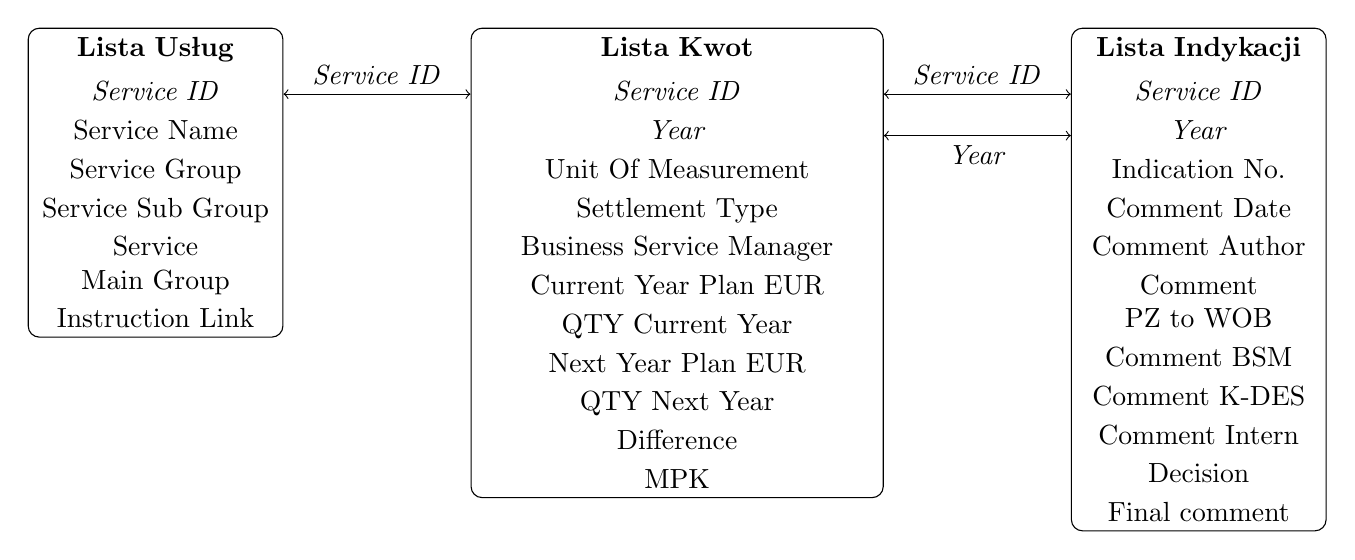
\begin{tikzpicture}

      \tikzstyle{ListBlock} = [
      rectangle,
      rounded corners,
      minimum width=3cm,
      minimum height=1cm,
      text centered,
      draw=black,
      fill=white,
      anchor=north
      ]

      \node (ListaUslug) [ListBlock, text width=3cm] at (0,0) {
        \textbf{Lista Usług}\\[4pt]
        \textit{Service ID}\\[2pt]
        Service Name\\[2pt]
        Service Group\\[2pt]
        Service Sub Group\\[2pt]
        Service Main Group\\[2pt]
        Instruction Link\\[2pt]
      };

      \node (ListaKwot) [ListBlock, text width=5cm]
      at ([xshift=5cm] ListaUslug.north east) {
        \textbf{Lista Kwot}\\[4pt]
        \textit{Service ID}\\[2pt]
        \textit{Year}\\[2pt]
        Unit Of Measurement\\[2pt]
        Settlement Type\\[2pt]
        Business Service Manager\\[2pt]
        Current Year Plan EUR\\[2pt]
        QTY Current Year\\[2pt]
        Next Year Plan EUR\\[2pt]
        QTY Next Year\\[2pt]
        Difference\\[2pt]
        MPK\\[2pt]
      };

      \node (ListaIndykacji) [ListBlock, text width=3cm]
      at ([xshift=4cm] ListaKwot.north east) {
        \textbf{Lista Indykacji}\\[4pt]
        \textit{Service ID}\\[2pt]
        \textit{Year}\\[2pt]
        Indication No.\\[2pt]
        Comment Date\\[2pt]
        Comment Author\\[2pt]
        Comment PZ to WOB\\[2pt]
        Comment BSM\\[2pt]
        Comment K-DES\\[2pt]
        Comment Intern\\[2pt]
        Decision\\[2pt]
        Final comment\\[2pt]
      };

      \draw [<->] ([yshift=-2em-4pt]ListaUslug.north east) -- node[anchor=south]{\textit{Service ID}} ([yshift=-2em-4pt]ListaKwot.north west);
      \draw [<->] ([yshift=-2em-4pt]ListaKwot.north east) -- node[anchor=south]{\textit{Service ID}} ([yshift=-2em-4pt]ListaIndykacji.north west);
      \draw [<->] ([yshift=-3.5em-4pt]ListaKwot.north east) -- node[anchor=north]{\textit{Year}} ([yshift=-3.5em-4pt]ListaIndykacji.north west);

    \end{tikzpicture}}
  \caption{Schemat relacji między listami.}
  \label{SchematList}
\end{figure}

Model danych przedstawiony na Rysunku \ref{SchematList} został zaprojektowany z uwzględnieniem następujących założeń:

\begin{itemize}
  \item \emph{Lista usług} pełni rolę centralnego rejestru serwisów, zawierając ich podstawową charakterystykę,
  \item \emph{Lista kwot} umożliwia śledzenie zmian w wymiarze finansowym na przestrzeni lat,
  \item \emph{Lista indykacji} przechowuje historię procesu decyzyjnego wraz z towarzyszącymi komentarzami i ustaleniami.
\end{itemize}



